\documentclass{beamer}
\usetheme{CambridgeUS}

\usepackage[czech]{babel}
\usepackage[utf8]{inputenc}
\usepackage[T1]{fontenc}

\usepackage{graphics}
%\usepackage{multicol}

\providecommand{\uv}[1]{\quotedblbase #1\textquotedblleft}

\author{Róbert Kolcún, xkoclu00}
\title{Typografie a publikování\,--\,5.\,projekt}
\subtitle{Vývoj tankov}

\institute{VUT v~Brně \\FIT}
\date{\today}

\begin{document}
	\begin{frame}
		\maketitle
	\end{frame}
	
	\begin{frame}
		\frametitle{História}
		\begin{itemize}
			\item Starovek --\ katapulty, balisty, staroveké bojové vozy a slony
			\item Novovek --\ prvý návrh tanku, Leonardo da Vinci okolo roku 1500
			\item Rok 1878 --\ revolučná myšlienka v článku od plukovníka C.B.Brackenburyho o delostrelectve ako útočnej sile pod pancierom
			\item 19.stor --\ vynález spaľovacieho motora $\Rightarrow$ vhodný pohon pre tanky
			\item Prelom 19. a 20.stor --\ obrnené automobily a vývoj pásov pre poľnohospodárske stroje
			\item Leto 1915 – prvý kompletný prototyp tanku pod menom „Little Willie“
		\end{itemize}
	\end{frame}
	
	
	
	\begin{frame}
		\frametitle{Tank vstupuje do vojny}
		\begin{itemize}
			\item Júl 1916 --\ britské jednotny útočia na nemecké na rieke Somme
			\item Začiatok jednej z najväčších a najkrvavejších bitiek 1.Svetovej vojny
			\item Rozhodnutie Britského velenia o nasadenie asi 50 tankov
			\item 15.September --\ tanky ukazujú svoju silu, prenikajú do nemeckých línií
		\end{itemize}
		
		\begin{block}{Osud 49 tankov}
			7 nedorazilo, 9 sa pokazilo, 5 uviazlo v priekope, 9 zaostalo \\ zo zvyšných len 9 dokázalo splniť svoju úlohu \uv{na plno}
		\end{block}
	\end{frame}
	
	
	
	\begin{frame}
		\frametitle{Tanky 1.Svetovej vojny}
		\begin{columns}
			\column{0.5\textwidth}
				\begin{itemize}
					\item Maximálna rýchlosť tankov:
					\begin{itemize}
						\item 8km/h pri \textit{Markoch}
						\item 12km/h pri \textit{St. Chamond}
					\end{itemize}
					\smallskip
					\item Technické problémy
					\begin{itemize}
						\item priechodnosť terénu bola slabá
						\item pancier nemal záchytnú vrstvu
						\item poruchovosť tankov --\ 1918 proti Nemecku až 90\,\%
					\end{itemize}
				\end{itemize}
				
			\column{0.5\textwidth}
				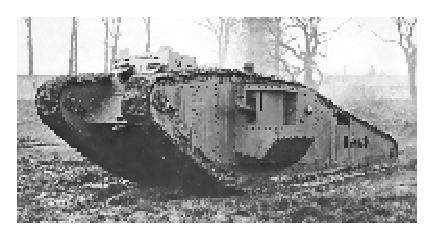
\includegraphics[scale=0.8]{mark} \\
				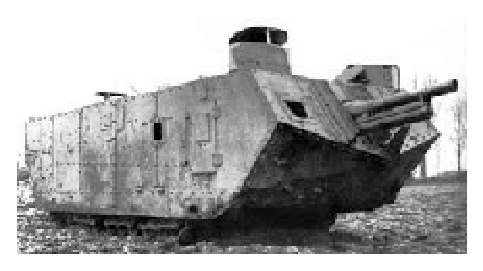
\includegraphics[scale=0.512]{stchamond}
		\end{columns}
	\end{frame}
	
	
	
	\begin{frame}
		\frametitle{Medzivojnové obdobie}
		\begin{itemize}
			\item britské tankové armády boli rozpustené, no vyvoj sa nezastavil
			\item britske modely tankov tvorili zaklad vývoju tankov v iných krajinách.
			\item francúzi disponovali cca 6000 tankami, boli najmocnejšou tankovou veľmocou na svete
			\item ZSSR roku 1995 začala vývoj najslávnejšieho a najúspeśnejśieho tanku T-34
			\item nástupom Adolfa Hitlera, ktorý Versaillsku zmluvu ignoroval, sa začala tanková revolúcia v nemecku
		\end{itemize}
	\end{frame}
	
	
	
	\begin{frame}
		\begin{table}
			\frametitle{Najpoužívanejšie tanky 2.Svetovej vojny}
			\small
			\begin{tabular}{l | c | c | c | c }
				Názov tanku 			& Kanón	& Guľomet(mm) 	& Max.rýchlosť 	& Vyrobených	\\
				\hline \hline
				Pzkpf. IV 				& 75 mm		& MG 34 -\ 7,92 & 40 km/h	& 9000		\\ 
				Pzkpf. V \uv{Panther}	& 75 mm		& MG 34 -\ 7,92 & 46 km/h	& 4800		\\
				Pzkpf. VI \uv{Tiger} 	& 88 mm		& MG 34 -\ 7,92 & 38 km/h	& 1354		\\
				\hline	
				KV-1 					& 76,2 mm	& DT -\ 7,62 	& 35 km/h	& 2553		\\
				T-34 					& 76,2 mm	& DT -\ 7,62 	& 55 km/h	& >60000	\\
				\hline
				M10 Wolwerine			& 76 mm		& M2HB -\ 12,7 	& 51 km/h	& 4993	\\
				M4 Sherman				& 75 mm		& M2HB -\ 12,7 	& 39 km/h	& 49234		\\
				\hline
				A22 Churchill			& 57 mm		& BESA -\ 7,62 	& 25 km/h	& >300		\\
			\end{tabular}
			\caption{Výrobne špeficikácie tankov}
		\end{table}
	\end{frame}
	
	
	
	\begin{frame}
		\frametitle{Zaujímavé prototypy tankov 2.Svetovej vojny}
		\begin{columns}
			\column{0.5\textwidth}
			\begin{itemize}
				\item \textit{Lankreuzer P.1000 (Nemecko)}
				\begin{itemize}
					\item extrémne ťažký tank
					\item 1943 bol projekt zastavený a žiaden tank sa nikdy nevyrobil
					\item mal byť vyzbrojený námornými delami
					\item verí sa, že vežu postavili a použili ako pozemnú delostreleckú batériu
				\end{itemize}
				
				\item \textit{O-I (Japonsko)}
				\begin{itemize}
					\item super ťažký tank
					\item vraj bol postavený v roku 1944 a neskôr poslaný do Mandžuska
				\end{itemize}
			\end{itemize}
			
			\column{0.5\textwidth}
				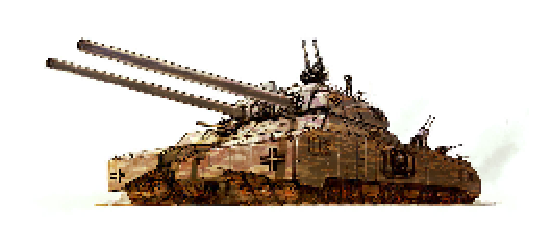
\includegraphics[scale=0.65]{potkan} \\
				
\includegraphics[scale=0.75]{oi}
		\end{columns}
	\end{frame}
	
	
	
	\begin{frame}
		\frametitle{Tanky súčastnosti}
		\begin{columns}
			\column{0.5\textwidth}
			\begin{itemize}
				\item dnes tanky obsahujú npr.:
				\begin{itemize}
					\item inteligentne bojové systémy
					\item automaticky navádzané rakety
					\item moderné pancierové systémy
				\end{itemize}
				\item dnes sa používaju tanky 3.generácie
				\item 4.generácia by sa už mala dostávať do výroby
				\item príchod 5.generácie sa odhaduje na rok 2020 \linebreak \textit{(Poľský tank PL --\ 01)}
			\end{itemize}
			
			\column{0.5\textwidth}
			\begin{block}{Prototyp 5.generácie \textit{PL --\ 01}}
				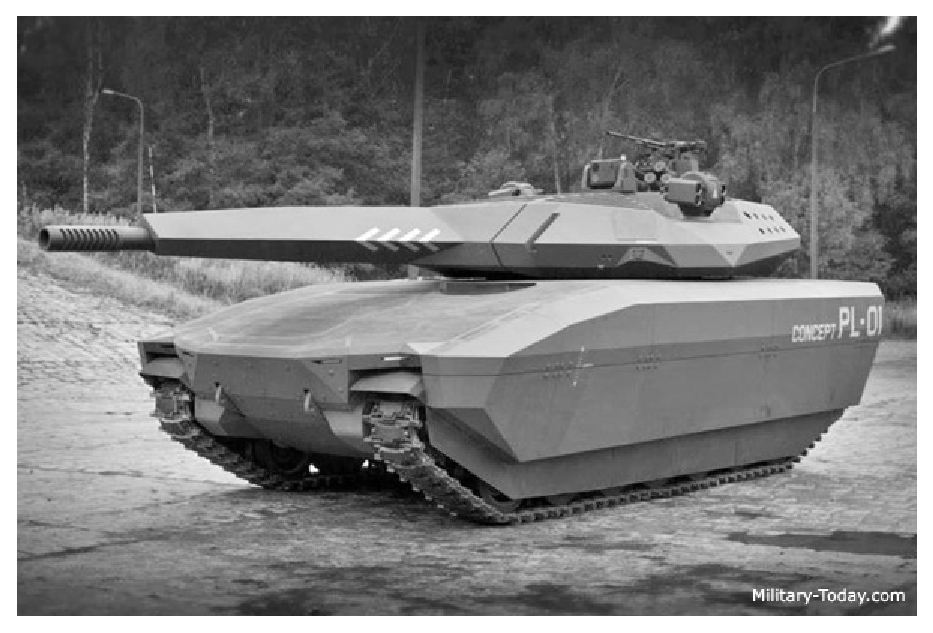
\includegraphics[scale=0.4]{pl01}
			\end{block}
		\end{columns}
	\end{frame}
	
	
	
	\begin{frame}
		\frametitle{Použíté zdroje}
		\footnotesize
		\begin{itemize}
			\item \url{https://sk.wikipedia.org/wiki/Dejiny_tankov}
			\item \url{http://www.historyweb.sk/clanky/detail/ako-tanky-nahradili-kone}
			\item \url{http://www.techportal.sk/armada/146-vznik-a-vyvoj-tankov-as-2-medzivojnove-obdobie}
			\item \url{http://sk.wikipedia.org/wiki/KV-1}
			\item \url{http://sk.wikipedia.org/wiki/T-34}
			\item \url{http://sk.wikipedia.org/wiki/M10_Wolverine}
			\item \url{http://sk.wikipedia.org/wiki/M4_Sherman}
			\item \url{http://sk.wikipedia.org/wiki/A22_Churchill}
			\item \url{http://sk.wikipedia.org/wiki/PzKpfw_IV}
			\item \url{http://sk.wikipedia.org/wiki/Panther_(tank)}
			\item \url{http://sk.wikipedia.org/wiki/PzkpfwVI_Tiger}
			\item \url{http://en.wikipedia.org/wiki/O-I}
			\item \url{http://sk.wikipedia.org/wiki/Landkreuzer_P._1000_Ratte}
		\end{itemize}
	\end{frame}
	
\end{document}
